\documentclass{article}
\usepackage{amsmath}
\usepackage{soul}
\usepackage{graphicx}
\usepackage{subcaption}
\graphicspath{ {./images/} }

\newcommand{\units}[1]{\texttt{#1}}
\newcommand{\biggbreak}{\\[1ex]}
\usepackage[margin=1.5cm]{geometry}


\usepackage{fancyhdr}

\pagestyle{fancy}
\fancyhf{}
\rhead{qwrx21}
\lhead{Report}
\rfoot{\thepage}
  
\begin{document}

All data was collected from runs on a Hamilton par7.q node.

Figure [Fig.\ref{fig:scaling}] shows the scaling characteristics of step 4 in terms of the number of bodies. 
We see from [Fig.\ref{fig:scaling_sub}] that scenarios with over 1000 bodies scale well to Hamilton's 24 cores, whereas models using $<$1000 bodies scale less well. 
If we assume this is a strong scaling model, following $t(p) = f \cdot t(1) + (1-f)\cdot \frac{t(1)}{p}$, we can calculate constant $f$ for each data point [Fig.\ref{fig:scaling_f}]. We can see scenarios with $>=500$ bodies are modeled well by the strong scaling model as there is a low variance of $f$ estimations, giving evidence that $f$ is a constant. 
However, the strong scaling model breaks down under $500$ bodies as $f$ is likely not constant. 
I suspect this breakdown is caused by the overhead for OMP to create and synchronize threads. 
This overhead is likely a function of the number of threads and could explain the speedup then slowdown for $200$ bodies.
We also see that $f$ decreases with more bodies. In my implementation some of the calculations with runtime $O(n)$ are done in series (where $n$ is number of bodies); However, all calculations with runtime $O(n^2)$ are done in parallel. Hence we would expect f to decrease as $O(n^2)$ dominates.

\begin{figure}[h!]
  \begin{center}
  \begin{subfigure}{.5\textwidth}
    \begin{center}
  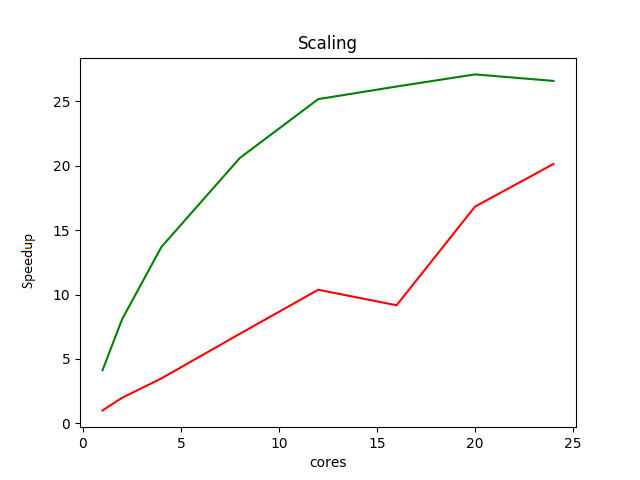
\includegraphics[width=.95\textwidth]{scaling.png}
  \caption{}
  \label{fig:scaling_sub}
\end{center}
  \end{subfigure}%
  \begin{subfigure}{.5\textwidth}
    \begin{center}
    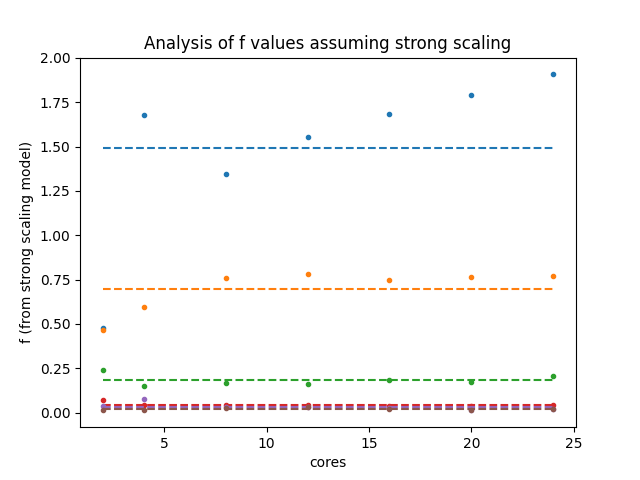
\includegraphics[width=.95\textwidth]{f.png}
    \caption{}
    \label{fig:scaling_f}
  \end{center}
    \end{subfigure}%
    \caption{Scaling and f calculation for step 4.}
  \label{fig:scaling}
\end{center}
\end{figure}

We see that both step 1 and step 3 converge as evident by parallel lines between both experiments for each method (step 1, step 3) trending towards 0 [Fig.\ref{fig:convergence}] From these lines we can calculate the approximate converge order for each step using their gradient. We see that step 1 has approximate convergence order $1.76$ and $1.84$; step 3 approximate convergence order $3.02$ and $2.86$. These approximate experimental converge orders match closely with the theoretical convergence values. Step 1, using Euler's method, has a theoretical convergence order $O(h^2)$ and step 3, using RK(2), $O(h^3)$. 


\begin{figure}[h!]
  \begin{center}
  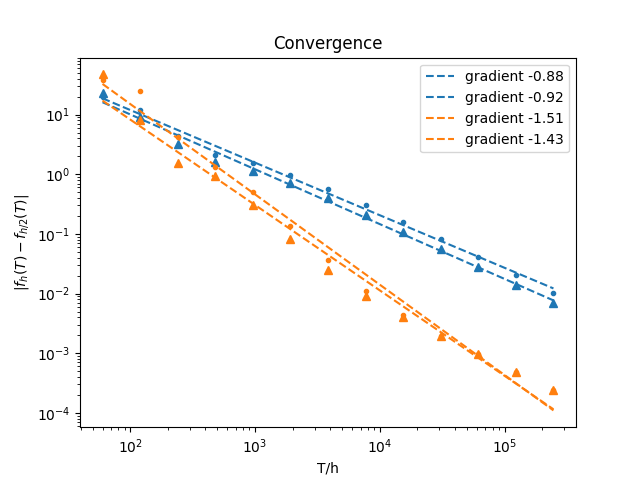
\includegraphics[scale=0.6]{convergence.png}
    \caption{step 1 (blue) step 3 (orange). Change in errors for a 2 body system under extreme conditions (near collision).}
    \label{fig:convergence}
  \end{center}
  \end{figure}


 

\end{document}


